% !TEX root = ../ITGO.tex

\subsection*{Welded beam design problem}


The welded beam design \citep{WB} is the problem of minimizing the fabrication cost of a welded beam, subject to seven inequality constraints, being two linear and five nonlinear. The constraints include shear stress ($\tau$), bending stress in the beam ($\sigma$), buckling load on the bar ($Pc$), end deflection on the beam ($\delta$) and some more side constraints. The four design variables are continuous. The feasible best known objective value is $f(\bm{x}^*) = 1.7248523$. Figure \ref{fig:WB} presents the schematic of the welded beam design problem. \\


\begin{figure}[h]
    \begin{center}
    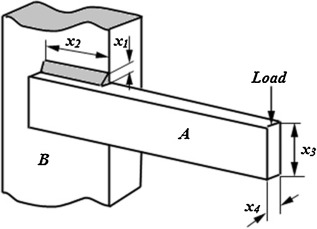
\includegraphics[scale=0.7]{Imgs/WB.jpg}
    \end{center}
    \captionsetup{justification=centering}
    \caption{Schematic view of the welded beam design problem.}\label{fig:WB}
\end{figure}


\prob{Appendix/Problems/WB}